\documentclass[]{article}
\usepackage{amsmath}
\usepackage[utf8]{inputenc}
\usepackage[italian]{babel}
\usepackage[T1]{fontenc}
\usepackage{indentfirst}
\usepackage{array}
\usepackage{titlesec}
\usepackage{multicol}
\usepackage{graphicx}
\usepackage{float}
\usepackage{listings}
\graphicspath{ {./Immagini/} }
\titleformat{\subsection}[runin]{\normalfont\bfseries}{\thesubsection}{0.5em}{}

\def\code#1{\texttt{#1}} % defines new command for some monospace font text

% Margins
\addtolength{\textwidth}{1.0in}
\addtolength{\textheight}{2.0in}
\addtolength{\evensidemargin}{-0.75in}
\addtolength{\oddsidemargin}{-0.75in}
\addtolength{\topmargin}{-1.0in}


\begin{document}


% Title & author
\title{Esercizio F: Componenti connesse e MST}
\author{Giovanni Stefanini - 6182949}
\date{Maggio 2021}
\maketitle

% Introduzione
\section*{Introduzione}
Analisi delle performance di un'implementazione in Python della struttura dati Union-Find e degli algoritmi per il calcolo delle componenti connesse e di un albero di connessione minimo di un grafo.\\

% Union-Find
\section {Union-Find}
La {\bf Union-Find} è una struttura dati in grado di gestire una collezione $S = \{ S_1, S_2, ..., S_k \}$ di {\bf insiemi disgiunti dinamici}. Le operazioni consentite sono le seguenti:\\

\begingroup
\leftskip2em \rightskip2em
\noindent \code{MakeSet(x)}: crea un nuovo insieme $S_i = \{ x \}$ e aggiunge $S_i$ a $S$\\
\code{Union(x, y)}: aggiunge $S_x$ a $S_y$ e distrugge $S_x$ (o viceversa)\\
\code{FindSet(x)}: ritorna il rappresentante (la chiave) dell'insieme che contiene $x$
\par
\endgroup

\vspace{0.20in}

Il tempo di esecuzione per \code{MakeSet(x)} è $O(1)$, in quanto la funzione deve solo aggiornare dei puntatori. Diversamente accade per \code{FindSet(x)}, che potrebbe dover scorrere tutti gli elementi di $S$ prima di trovare $x$ (o restituire un $NIL$). \code{Union(x, y)} è invece ancora più costosa in quanto, nel caso peggiore, potrebbe dover unire tutti gli elementi in $S$, per un tempo di esecuzione quadratico $O(n^2)$.

% Componenti connesse
\section {Componenti connesse}
Le {\bf componenti connesse} di un grafo $G = (V,E)$ partizionano i vertici $V$ in classi di equivalenza secondo la relazione "è raggiungibile da'', ovvero per il grafo $G$ i vertici $u$ e $v$ sono nella stessa componente connessa se e solo se c'è un cammino tra di loro. L'algoritmo (in pseudocodice) per il loro calcolo è:\\

\begingroup
\leftskip2em \rightskip2em
\noindent \code{ConnectedComponents(G)}\\
\indent\code{for ogni vertice $v \in G.V$}\\
\indent\indent\code{MakeSet(v)}\\
\indent\code{for ogni arco $(u, v) \in G.E$}\\
\indent\indent\code{if FindSet(u) $\neq$ FindSet(v)}\\
\indent\indent\indent\code{Union(u,v)}
\par
\endgroup

% MST Kruskal
\section {Alberi di connessione minimi (MST)}
Gli alberi di connessione minimi, o {\bf MST} ({\em minimum spanning trees}), sono alberi (ovvero sottoinsiemi degli archi di un grafo $G = (V,E)$) che connettono tutti i vertici minimizzando il costo totale degli archi stessi (nei grafi pesati). Ogni MST di $G$ (ce ne possono essere più di uno) ha sempre $|V|-1$ archi e non contiene cicli (dato che si tratta di un albero, grafo aciclico non orientato per definizione). Per trovare un MST di $G$ si può utilizzare la struttura dati Union-Find in combinazione con uno tra gli algoritmi di Kruskal o Prim (entrambi con tempi di esecuzione dipendenti dall'implementazione di Union-Find). In questo esperimento faremo uso soltanto dell'algoritmo di Kruskal, qui illustrato in pseudocodice:\\

\begingroup
\leftskip2em \rightskip2em
\noindent \code{MST-Kruskal(G, w)}\\
\indent\code{$A = \emptyset$}\\
\indent\code{for ogni vertice $v \in G.V$}\\
\indent\indent\code{MakeSet(v)}\\
\indent\code{ordina gli archi di $G.E$ in ordine non decrescente rispetto al peso $w$}\\
\indent\code{for ogni arco $(u, v) \in G.E$ preso in ordine di peso non decrescente}\\
\indent\indent\code{if FindSet(u) $\neq$ FindSet(v)}\\
\indent\indent\indent\code{$A \leftarrow A \cup \{(u,v)\}$}\\
\indent\indent\indent\code{Union(u,v)}\\
\indent\code{return $A$}
\par
\endgroup

% Specifiche tecniche
\section {Specifiche tecniche}
Per la creazione del programma nel linguaggio Python sono state utilizzate le seguenti classi: \\

\code{\bf {-unionFind()}}:	Ai fini dell'esperimento, la struttura dati Union-Find è stata implementata come un dizionario $S$ in cui ogni chiave è costituita da un vertice del grafo, ed i suoi relativi valori sono gli archi che partono/entrano in esso (il grafo non è orientato). Tre funzioni, \code{makeSet(x)}, \code{union(x, y)} e \code{findSet(x)} (quest'ultima ritorna la chiave di $x$ oppure \code{None}), implementano nella struttura S gli algoritmi sopra presentati in pseudocodice. \\

\code{\bf {-node(k)}}: Classe ausiliaria per la rappresentazione dei vertici; contiene soltanto la chiave $k$ del vertice. \\

\code{\bf {-edge(u, v, w)}}: Classe ausiliaria per la rappresentazione degli archi $(u,v)$, contenente i nodi $u$ e $v$ ed il peso $w$ dell'arco (sempre $1$ in grafi non pesati). \\

\code{\bf {-randomGraph(n, min, max, w)}}: Classe che genera un grafo casuale, con la possibilità di scegliere il numero di nodi $n$ ed il numero minimo ($min$) e massimo ($max$) di archi. Dopo alcuni controlli sui valori ricevuti in input di $min$ e $max$ viene generato il numero $k$ di archi da creare, compreso tra $min$ e $n\cdot max$ (in modo che $k$ sia almeno $0$ ed al più $n\cdot n$); un ciclo \code{while} genera i $k$ archi aggiungendoli alla matrice di adiacenza $adjMatrix$ del grafo, che era stata precedentemente inizializzata a tutti zeri. Se il grafo non è pesato ($w = False$), allora gli archi aggiunti avranno tutti peso pari a $1$; altrimenti, se $w = True$, gli archi avranno un peso scelto casualmente tra $1$ e $15$ (valori arbitrari). In seguito viene creata la lista dei nodi $nodes$ e quella degli archi $edges$, quest'ultima analizzando la presenza degli archi in $adjMatrix$. Due funzioni aggiuntive, \code{MSTKruskal()} e \code{connectedComponents()} implementano sul grafo gli omonimi algoritmi, seguendo letteralmente lo pseudocodice sopra illustrato. \\

Il programma principale di Test ({\em Test3ASD.py}) crea, in cicli \code{for}, grafi casuali pesati e non, con un numero di nodi sempre maggiore (fino ad un massimo di $n = 450$, con step di 30), e calcola per ognuno di essi le componenti connesse ed un albero minimo di connessione tramite le funzioni \code{connectedComponents()} e \code{MSTKruskal()} di \code{randomGraph(n, min, max, w)}. Per ogni iterazione dei suddetti algoritmi viene salvato il tempo di esecuzione in array ausiliari, ai fini di tracciare successivamente i grafici e le tabelle {\em tabella-GrafiNONPesati.html} e {\em tabella-GrafiPesati.html} (che elencano i risultati), utili per l'analisi delle performance.\\

Le {\bf specifiche hardware e software} della macchina utilizzata per eseguire i test sono:\\

\begingroup
\leftskip2em \rightskip2em
\noindent {\bf Scheda madre}: X580VD Scheda di base ASUSTeK COMPUTER INC.\\
{\bf CPU}:  Intel Core i7-7700HQ CPU - 2.80GHz, 2808 Mhz, 4 core, 8 processori logici\\
{\bf RAM}: 16 GB\\
{\bf SSD}: SanDisck SD8SN8U128G1002 - 120 GB\\
{\bf HDD}: TOSHIBA MQ04ABF100 - 1 TB\\
{\bf SO}: Microsoft Windows 10 Home \\
{\bf IDE}: JupyterLab 2.2.6 \\
\vspace{-5mm}


% Prestazioni attese
\section*{Prestazioni attese}
Considerato il tempo di esecuzione $O(n^2)$ di \code{Union(x, y)}, che rende quadratici gli algoritmi per il calcolo delle componenti connesse e di un albero minimo di connessione, ci si aspetta che gli andamenti, all'aumentare dei nodi, possano essere sempre più simili a una funzione quadratica (i.e. una parabola), e che i tempi di esecuzione siano quindi sempre maggiori.

% Analisi dei risultati
\section {Analisi dei risultati}
\vspace{-5mm}

\begin{figure}[!h]
\centering
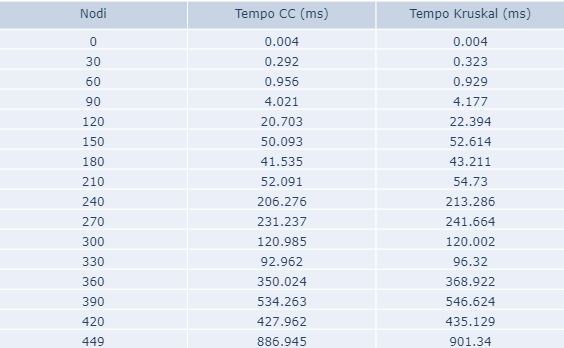
\includegraphics[width=\textwidth]{tabella_GrafiNONPesati}
\caption{Tabella del tempo $t$ ($s$) delle CC e di MST-Kruskal per alcuni grafi non pesati $G$}
\label{fig:fig1}
\end{figure}

{\bf GRAFI NON PESATI}: Osservando la prima tabella (fig.\ref{fig:fig1}) e i due grafici (fig.\ref{fig:fig2}), riferiti ai grafi non pesati, è abbastanza chiara la conferma delle aspettative riguardo i tempi di esecuzione: \code{union(x, y)} richiede proprio $O(n^2)$, portando ad avere, a meno delle imperfezioni dovute ad un numero crescente di nodi ed uno sempre maggiore (ma comunque variabile) di archi, un andamento del tempo che possiamo immaginare sia una curva quadratica o, per meglio dire, una parabola. È interessante, inoltre, notare un aspetto non molto evidente, ma molto importante: la colonna sulla destra, riferita ai tempi di esecuzione di \code{MSTKruskal()}, è quasi perfettamente identica a quella a sinistra, riferita ai tempi di \code{connectedComponents()}. \\
Questo fenomeno non è affatto casuale, in quanto si è continuamente ripresentato durante i test condotti (non solo quindi nell'istanza da cui sono state tratte le figure); esso è dovuto al fatto che i due algoritmi analizzati sono estremamente simili, al punto da far coincidere, nella pratica, i loro tempi di esecuzione. Tuttavia, studiando la tabella, si nota come \code{MSTKruskal()} ha sempre un tempo lievemente superiore rispetto a \code{connectedComponents()}, dovuto alle poche righe di codice aggiuntive che questo algoritmo richiede.\\

\begin{figure}[H]
\centering
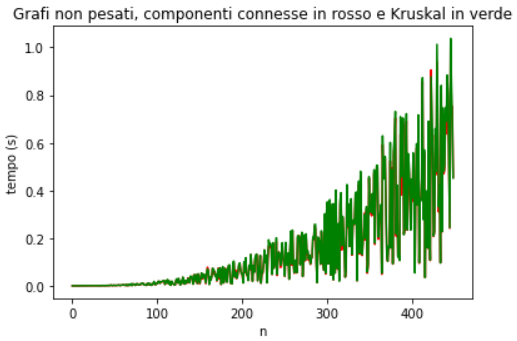
\includegraphics[width=.7\textwidth, height=.6\textheight, keepaspectratio]{GraficoGrafiNonPesatiCCeK}
\caption{Grafici del tempo $t$ ($s$) delle CC e di MST-Kruskal per alcuni grafi non pesati}
\label{fig:fig2}
\end{figure}



\begin{figure}[!h]
\centering
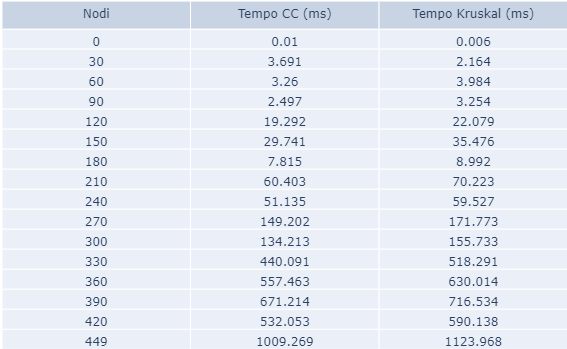
\includegraphics[width=\textwidth]{tabella_GrafiPesati}
\vspace{-5mm}
\caption{Tabella del tempo $t$ ($s$) delle CC e di MST-Kruskal per alcuni grafi pesati $G$}
\label{fig:fig3}
\end{figure}

{\bf GRAFI PESATI}: Proseguendo con i grafi pesati, si osserva (fig.\ref{fig:fig3} e fig.\ref{fig:fig4}) che accadono gli stessi fenomeni descritti per i grafi non pesati, sia per quanto riguarda la quadraticità del tempo di esecuzione di \code{union(x, y)}, sia per quanto riguarda la quasi completa sovrapposizione dei tempi di esecuzione di \code{connectedComponents()} e \code{MSTKruskal()}. L'unica differenza, visibile nella rispettiva tabella  (fig. \ref{fig:fig2}), consiste nei tempi di esecuzione generalmente maggiori, dovuti all'elaborazione di nodi contenenti più informazioni rispetto ai grafi non pesati e, nel caso del calcolo di un MST, all'ordinamento degli archi (il quale avrà più lavoro da svolgere, dati i pesi diversi).

\begin{figure}[H]
\centering
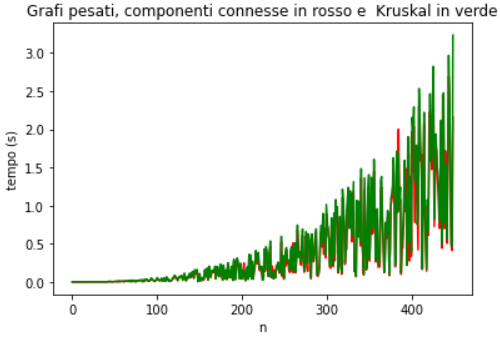
\includegraphics[width=.7\textwidth, height=.6\textheight, keepaspectratio]{GraficoGrafiPesatiCCeK}
\caption{Grafici del tempo $t$ ($s$) delle CC e di MST-Kruskal per alcuni grafi non pesati}
\label{fig:fig4}
\end{figure}


% Conclusioni
\section {Conclusioni}
In conclusione, l'implementazione di Union-Find in Python tramite un dizionario $S$ non permette di ottenere tempi di esecuzione migliori di $O(n^2)$ nel caso peggiore, e gli esperimenti condotti sui grafi hanno reso palese questo fatto. In ogni caso, sono stati confermati tramite gli esperimenti condotti i tempi di esecuzione quadratici di Union-Find (e \code{ConnectedComponents(G)} e \code{MST-Kruskal(G, w)} di conseguenza), e l'estrema somiglianza tra gli algoritmi trattati.

\end{document}
